\documentclass[a4paper,10pt]{article}
\usepackage[utf8]{inputenc}
\usepackage{graphics}
%opening
\title{Análisis numérico \\ Proyecto final \\ Resolución de la ecuación de Laplace en 2D.}
\author{Jean Pierre Pacheco Avila}

\begin{document}

\maketitle
\section{Introducción}

La ecuacion de Laplace es una ecuación en derivadas parciales y puede ser escrita de la siguiente forma:
$$ \frac{\partial^{2}u}{\partial^{2}x} + \frac{\partial^{2}u}{\partial^{2}y} = 0 $$ o también:
$$ \bigtriangledown^{2}u = 0$$ donde $ \bigtriangledown^{2} $ es el operador de Laplace o laplaciano. Esta ecuación es de suma
importancia ya que aparece en distintas ramas tales como astronomía, la electroestática, mecánica de fluidos, etc. Recibe el nombre en
honor al físico y matemático Pierre-Simon Laplace.


\section{Método de diferencias finitas}

Para reesolver la ecuación necesitamos encontrar la función $ u(x,y) $ que satisfaga la igualdad. Pero nosotros queremos 
resolverla de forma numérica, y además en esta ecuación aparecen las segundas derivadas, por lo que se usará el método de 
diferencias finitas para aproximar la solución. \\
Dado que nuestro dominio en este caso es un conjunto $ D \subset R^{2} $, y el método de diferencias finitas
requiere o hace uso de una partición del dominio, en este caso, necesitamos particionar tanto al eje X como al eje Y, por lo que
la partición de nuestro dominio se verá como un rectangulo cuadriculado. \\

Si la longitud de las particiones en X e Y son $\bigtriangleup x$ y $\bigtriangleup y$ respectivamente, entonces podemos escribir
la ecuación $$ \frac{\partial^{2}u}{\partial^{2}x} + \frac{\partial^{2}u}{\partial^{2}y} = 0 $$ como sigue, usando la formula
de diferencias finitas para aproximar la segunda derivada de $u$ en cada punto $ (x_{j},y_{i}) $ dentro de nuestro dominio obtenemos:
$$ \frac {u_{i+1,j} - 2u_{i,j} + u_{i-1,j}}{(\bigtriangleup x)^{2}} + \frac {u_{i,j+1} - 2u_{i,j} + u_{i,j-1}}{(\bigtriangleup y)^{2}} = 0$$

Si suponemos que $ \bigtriangleup x = \bigtriangleup y$ entonces obtenemos la siguiente ecuacion:
$$ -4u_{i,j} - u_{i+1,j} + u_{i-1,j}+ u_{i,j+1}+ u_{i,j-1}  = 0$$ donde $$ u_{i,j} = u(x_{j},y_{i}) $$
Así, obtendremos una ecuación por cada punto dentro del dominio discretizado, es decir, una ecuación para cada punto en nuestro
rectángulo.

Si despejamos $ u_{i,j}$ obtendremos:
$$ u_{i,j}  = \frac{u_{i+1,j} + u_{i-1,j}+ u_{i,j+1}+ u_{i,j-1}}{4} $$
Lo cuál indica que el valor de la función $u(xj,yi)$  es un promedio de los puntos a su alrededor. 
Pero para encontrar todos estos valores
debemos resolver un sistema de ecuaciones, un sistema de $ n x n $ donde $n = \# particiones en x  * \# numero de particiones en y $
\\
Un gráfico para una solución a la ecuación de Laplace en 2D es la siguiente:
\section{Gráfico}

\begin{figure}[htb]
\centering
 \scalebox{.6}{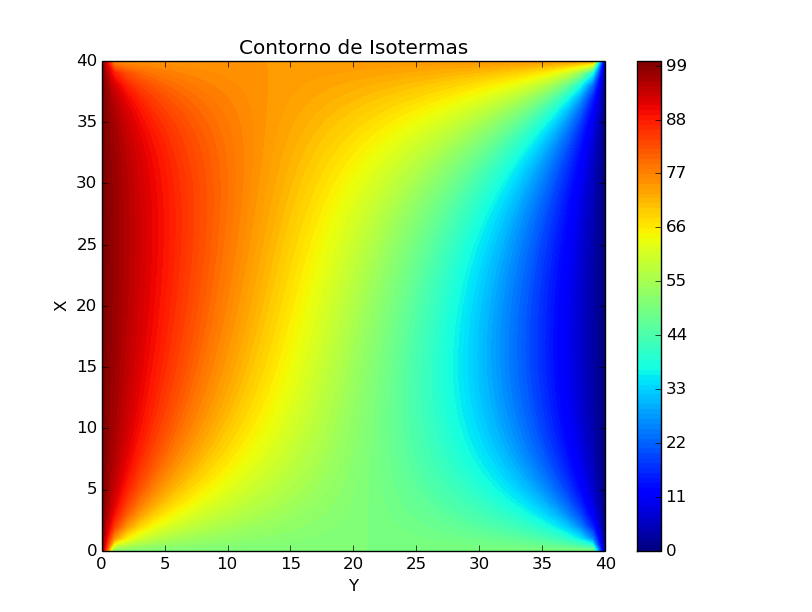
\includegraphics{figure.png}}
  \caption{Ejemplo}
\end{figure}

\end{document}
